\documentclass[12pt]{article}


\usepackage{amsmath,amssymb,amsthm,enumerate,graphicx}
\usepackage{ifthen,latexsym,syntonly}
\usepackage{setspace}
\usepackage[showrefs]{refcheck}  %use this to show equation and section labels
\usepackage[round,comma,authoryear]{natbib}   % for natbib
\usepackage{subfigure}
\usepackage{float}
\usepackage{epstopdf}
\usepackage{bm}
\usepackage{soul}

%commands to allow for easy editing
\usepackage[usenames,dvipsnames]{color}

%command to insert editing comments or track changes
\newcommand{\dge}[1]{\textcolor{blue}{$^{\textrm{dge}}${#1}}}
\newcommand{\apb}[1]{\textcolor{green}{$^{\textrm{apb}}${#1}}}
\newcommand{\tsj}[1]{\textcolor{red}{$^{\textrm{tsj}}${#1}}}

\bibliographystyle{mynat}


\onehalfspacing


   % for natbib
%\bibpunct{(}{)}{,}{a}{}{,}  % for natbib
%                            % need to have mynat.bst in an accesssible directory


\bibpunct{(}{)}{,}{a}{}{,}  % for natbib
                            % need to have mynat.bst in an accesssible directory

\newcommand{\EE}{\mathbb E}
\newtheorem{theorem}{Theorem}[section]
\newtheorem{remark}[theorem]{Remark}
\newtheorem{assumption}[theorem]{Assumption}
%\newtheorem{case}[theorem]{Case}
\newtheorem{claim}[theorem]{Claim}
%\newtheorem{conclusion}[theorem]{Conclusion}
\newtheorem{corollary}[theorem]{Corollary}
\newtheorem{condition}[theorem]{Condition}
\newtheorem{criterion}[theorem]{Criterion}
\newtheorem{definition}[theorem]{Definition}
\newtheorem{example}[theorem]{Example}
\newtheorem{lemma}[theorem]{Lemma}
\newtheorem{problem}[theorem]{Problem}
\newtheorem{proposition}[theorem]{Proposition}
%\newtheorem{solution}[theorem]{Solution}
%\newtheorem{summary}[theorem]{Summary}
\newtheorem{thm}[theorem]{Theorem}



\setlength{\oddsidemargin}{.05in} \setlength{\topmargin}{-.45in}
\setlength{\textwidth}{6.4in} \setlength{\textheight}{8.5in}


%\pagestyle{empty}

\title {Optimal Taxation with Incomplete Markets}
%\author{Anmol Bhandari, David Evans, Mikhail Golosov, Thomas J. Sargent}
\author{\textbf{Anmol Bhandari}\\apb296@nyu.edu \and \textbf{David Evans} \\ \texttt{dgevans@nyu.edu} \and \textbf{Mikhail Golosov}\\\texttt{golosov@princeton.edu} \and \textbf{Thomas J. Sargent} \\ \texttt{thomas.sargent@nyu.edu}
}

\begin{document}

\maketitle



\begin{abstract}

\end{abstract}


\noindent\textsc{Keywords:}
\section{Introduction}


\section{Environment}



We analyze economies that share the following features.
Government expenditures at time $t$, $g_t=g(s_t)$, and a productivity shock $\theta_t=\theta(s_t)$ are both functions of
  a Markov  shock $s_t\in \mathcal{S}$ having  $S \times S$ transition matrix $\Pi$ and initial condition $s_{-1}$.
   %; $g_t=g(s_t);\theta_t=\theta(s_t)$
An infinitely lived representative consumer has preferences over allocations  $\{c_t(s^t), l_t(s^t)\}_{t=0}^\infty$ of consumption and labor supply that are ordered
by
   \begin{equation*}
\mathbb{E}_{0}\sum_{t=0}^{\infty } \beta^t  U\left(
c(s^t),l(s^t)\right)  \label{utility lifetime}
\end{equation*}%
where $U$ satisfies \dge{(Not sure what we want to do here.  In all of our results we specialize to either CRRA or quasi-linear.)}.
  Labor produces output via the linear technology
  \begin{equation*}
  y_t=\theta_{t} l_{t} \end{equation*}
The representative consumer's tax bill
 at time $t \geq 0$ is
 \[- T_t + \tau_t \theta_{t}l_{t},  \ T_t \geq 0, \]
 where $\tau_t(s^t, b_{-1})$ is a flat rate tax on labor income and $T_t$ is a nonnegative transfer.
 Often, we'll set $T_t =0$.
The government and consumer trade a single  possibly risky  asset whose  time $t$ payoff $p_t$ is described by an $S \times S$ matrix $\mathbb{P}$:
\[p_t=\mathbb{P}(s_{t}|s_{t-1}).\]
Let $B_t$ denote the government's holdings of the asset and $b_t$ be the consumer's holdings.
Let $q_t= q_t(s^t; b_{-1})$ be the price of the single  asset at time $t$.
 At $t \geq 0$, the household's time budget constraint is
\[ c_{t}+b_{t}=\left( 1-\tau _{t}\right) \theta _{t}l_{t}+\frac{p_{t}}{q_{t-1}}b_{t-1}+T_{t}\] % \ T_t \geq 0$
 and the government's is
\[g_{t}+B_{t}+T_t=\tau _{t}\theta_{t}l_{t}+\frac{p_{t}}{q_{t-1}}B_{t-1}. \]
Feasible allocations satisfy
 \[c_{t}+g_t = \theta _{t} l_{t}, \ \forall t \geq 0 \]
Clearing in the time $t \geq 0$ market for the single asset requires
\[b_{t}+B_{t}=0. \]
Initial assets satisfy $b_{-1}=-B_{-1}$ An initial value of the exogenous state  $s_{-1}$ is given.
Equibrium objects including $\{c_t, l_t, \tau_t\}_{t=0}^\infty$ will come in the form of sequences of functions of  initial government debt  $b_{-1}$ and  $s^t = [s_t, s_{t-1}, \ldots, s_0, s_{-1}]$.


Borrowing from a standard boilerplate, we use the following:

\begin{definition}
An \textbf{allocation} is \dge{a sequence $\{c_t,l_t\}_{t=0}^\infty$ for consumption and labor}. A \textbf{price system} is a \dge{sequence of asset prices $\{q_t\}_{t=0}^\infty$}.  A \textbf{budget-feasible government policy} is \dge{a sequence of taxes, transfers and government asset holdings $\left\{ \tau _{t},T_{t},B_t\right\} _{t=0}^{\infty }$}
\end{definition}

\begin{definition}
Given  $\left(b_{-1}=-B_{-1},s_{-1}\right) $ and a government policy,  a \textbf{competitive equilibrium
with distorting taxes} is a price system, a budget-feasible government policy, and an allocation such that
the allocation is individually rational and the bond  market clears.
\end{definition}

\begin{definition}
Given $\left( b_{-1},B_{-1},s_{-1}\right) $, a \textbf{Ramsey plan} is a welfare-maximizing competitive
equilibrium with distorting taxes.
\end{definition}


\section{Two Ramsey problems}

Following \citet{LucasJr.1983}
and
\citet{Aiyagari2002}, we use a
``primal approach.''   To encode a  government policy and price system as a restriction on an allocation,
we  first obtain   the representative household's first order conditions:
\begin{subequations}
	\[
		U_{c,t} q_t = \beta \EE_t p_{t+1}U_{c,t+1}
	\]
	\[
		(1-\tau_t)\theta_tU_{c,t} = - U_{l,t}
	\]
\end{subequations}
We substitute these into the household's budget constraint to get a difference equation that we  solve forward   at every history for every $t \geq 0$.
That yields \textit{implementability constraints} on a Ramsey allocation that fall into two categories: (1) the time $t=0$ version is identical
with the {\em single} implementability constraint imposed by \citet{LucasJr.1983}; (2) the time $t \geq 1$ implementability constraints
are counterparts  of the additional
 \emph{measurability restrictions} that \citet{Aiyagari2002} impose on  a Ramsey allocation.
%
%\item[4.]  \textbf{Transfers: } We temporarily restrict transfers $T_t = 0$  $\forall t$. This is convenient for our analytical results.  We eventually show  that this assumption is not restrictive.
% \end{enumerate}





%
%The primal approach version of
%\begin{equation*}
%\max_{\{c_t,l_t\}} \EE_0\sum_{t=0}^\infty \beta^t U(c_t,l_t)
% \end{equation*}
% subject to
%
% \vspace{3mm}
%
% (a) \textbf{Feasibility}
%\begin{subequations}
%\begin{equation*}
%c_t + g_t = \theta_t l_t
% \end{equation*}
%
%(b) \textbf{Implementability constraint}
%
%% \begin{equation*}
%% \frac{b_{t-1}U_{c,t-1}}{\beta} = \frac{\EE_{t-1} p_t U_{c,t}}{p_t U_{c,t}}\EE_t\sum_{j=0}^\infty\beta^j\left( U_{c,t+j}c_{t+j}+U_{l,t+j}l_{t+j}\right)\text{  for $t\geq 1$ }
%% \end{equation*}
%\begin{equation*}
%b_{-1} = \frac1{U_{c,0}}\EE_0\sum_{t=0}^\infty \beta^t\left(U_{c,t}c_t+U_{l,t}l_t\right)
% \end{equation*}
%\end{subequations}
We first state our Ramsey problem, then Lucas and Stokey's.




\begin{problem}\label{prob:RamseyBEGS}
The  Ramsey problem is to choose an allocation and an appropriately measurable government debt sequence $\{b_t\}_{t=0}^\infty$ %sequences  functions
%$\{c_t(s^t),l_t(s^t), b_t(s^t)\}_{t=0}^\infty$
that attain:
\begin{equation}\label{eqn:Ramseyobj}
\max_{\{c_t,l_t,b_t\}} \EE_0\sum_{t=0}^\infty \beta^t U(c_t,l_t)
 \end{equation}
subject to
% \vspace{3mm}
%
% (a) \textbf{Feasibility}
\begin{subequations}
\begin{equation}\label{eqn:feas}
c_t + g_t = \theta_t l_t, \ t \geq 0
 \end{equation}

%(b) \textbf{Lucas-Stokey implementability constraint}
\begin{equation}\label{eqn:LSimplement}
b_{-1} = \frac1{U_{c,0}}\EE_0\sum_{t=0}^\infty \beta^t\left(U_{c,t}c_t+U_{l,t}l_t\right)
 \end{equation}

 %(c) \textbf{Measurability constraints}
 \begin{equation}\label{eqn:AMSSimplement}
 \frac{b_{t-1}U_{c,t-1}}{\beta} = \frac{\EE_{t-1} p_t U_{c,t}}{p_t U_{c,t}}\EE_t\sum_{j=0}^\infty\beta^j\left( U_{c,t+j}c_{t+j}+U_{l,t+j}l_{t+j}\right)\text{  for $t\geq 1$ }
 \end{equation}
\end{subequations}
\end{problem}

\begin{problem}\label{prob:RamseyLS}
Lucas and Stokey's Ramsey problem is to choose an allocation %$\{c_t(s^t),l_t(s^t)\}_{t=0}^\infty$
that attains % the maximum of
\begin{equation}\label{eqn:RamseyobjLS}
\max_{\{c_t,l_t\}} \EE_0\sum_{t=0}^\infty \beta^t U(c_t,l_t)
 \end{equation}
 subject to the single implementability constraint \eqref{eqn:LSimplement} and feasibility \eqref{eqn:feas} for all $t, s^t$.
\end{problem}

\begin{remark} Equation \eqref{eqn:feas} imposes feasibility, while equation  \eqref{eqn:LSimplement} is the single implementability constraint
present in \citet{LucasJr.1983}.  Equations \eqref{eqn:AMSSimplement} express  additional implementability constraints that comprise implementability constraints at every node from time $t \geq 1$. These generalize the \citet{Aiyagari2002} measurability constraints on a Ramsey allocation  to our more general payoff structure ${\mathbb P}$ for the
single asset. The measurability constraints \eqref{eqn:AMSSimplement}  are cast
in terms of the date, history $(t-1, s^{t-1})$ measurable state variable $b_{t-1}$ that for $t \geq 1$ is absent from Lucas and Stokey's complete markets Ramsey problem.  Evidently, Ramsey allocation for our incomplete markets economy automatically satisfies the single implementability constraint imposed by \citeauthor{LucasJr.1983}.
\end{remark}


\begin{remark}\label{rem:LSdebt}
State-contingent, but not history-dependent,  values of consumption, labor supply, and continuation government debt $\check b(s)$  solve the \citet{LucasJr.1983} Ramsey problem \ref{prob:RamseyLS}.  As intermediated by the Lagrange multiplier on the implementability constraint \eqref{eqn:LSimplement},
consumption, labor supply, and $\check b(s)$ are  functions of initial government debt $b_{-1}$ and the current state $s$, but not past
 $s$'s.
\end{remark}

\subsection{Motivation for  quasi-linear $U$\label{sec:excusequasilinear}}
Asymptotic properties of a Ramsey plan for our incomplete markets economy vary  with   asset returns that reflect
	properties of equilibrium prices $\{q_t(s^t|B_{-1},s_{-1})\}_t$ and the exogenous asset payoff matrix $\mathbb{P}$.  \dge{This is readily observed in equation \eqref{eqn:AMSSimplement}, where $U_{c,t}$ and $p_t$ enter in the same way.} 
To focus exclusively on the exogenous $\mathbb{P}$ part of returns, we begin  by studying an economy with  quasi-linear  utility function:
  \begin{equation}\label{eqn:UQL}
U(c,l)=c-\frac{l^{1+\gamma}}{1+\gamma},\end{equation}\dge{which sets $U_{c,t}= 1$.}  Asymptotic properties of a Ramsey plan for our incomplete markets economy vary  with   asset returns that reflect
	properties of equilibrium prices $\{q_t(s^t|B_{-1},s_{-1})\}_t$ and the exogenous asset payoff matrix $\mathbb{P}$.
This utility function pins down $q_t=\beta \mathbb{E}_t
\mathbb{P}(s_{t+1}|s_t)$.  After studying the consequences of quasi-linear utility, we shall Ramsey plans for utility functions that express risk aversion with respect to consumption and so activate fluctuating $q_t$.
	


\section{Quasi-linear preferences}

Throughout this section, we assume that $U$ is quasi-linear and use an indirect three step approach to  characterize  the asymptotic behavior of government  debt and the tax rate.
(1) Construct  an operator.
We pose the following problem:
\begin{problem}\label{prob:PPoperator}
 Given arbitrary initial government debt $b_{-1}$, what is an optimal asset payoff matrix?
\end{problem}
\noindent Problem \ref{prob:PPoperator} induces an operator that maps initial government debt $b_{-1}$ into an optimal payoff matrix $\mathbb{P^*}$ for the single asset:
\begin{equation}\label{eqn:PPoperator}
\mathbb{P}^* =\mathbb{P}^*(b_{-1}) .\end{equation}
\noindent (2) Apply the inverse of the operator $\mathbb{P}^*$.
For an arbitrary payoff matrix $\mathbb{P}$,  let
\begin{equation}\label{eqn:invPoperator}\mathbb{P}=\mathbb{P}^*(b^*) \ \textrm{or} \ b^* = \mathbb{P}^{* -1}(\mathbb{P}) .\end{equation}
For initial government debt $b_{-1} = b^*$, a Ramsey plan for the incomplete markets economy has $b_t = b^*$ for all $t \geq 0$.
(3) Starting from an arbitrary initial government $b_{-1}$ and an arbitrary payoff matrix $\mathbb{P}$,  establish conditions under  which $b_t \to b^*$ under a Ramsey plan.


In particular, where $S=2$ and shocks $s_t$ are IID,  we describe a large set of  $\mathbb{P}$'s for which government debt $b_t$  under a Ramsey plan converges to $b^*$ that solves \eqref{eqn:invPoperator}.
%	\[\mathbb{P}=\mathbb{P}^*(b^*)\]
 For more general shock processes, we numerically find  an ergodic set of $b_t$'s
 hovering around a debt level $\tilde b$;    The optimal $\mathbb{P}^*$ associated with $\tilde b$ approximates $\mathbb{P}$ \dge{(Given how important this is it is probably worth a week trying to nail this down a bit more)}:
	\[\mathbb{P}\approx \mathbb{P}^*(\tilde b)\]
%	\textcolor{red}{Anmol and David XXXXXX: the preceding approximate equality needs clarification at least for me. What does it mean?}
	

Here is how we execute these three steps.
(1)
  Given $b_{-1}$, solve problem \ref{prob:RamseyLS} to compute a  Lucas-Stokey Ramsey allocation.
(2) Note that \citeauthor{Aiyagari2002}-like measurability constraints \eqref{eqn:AMSSimplement} are invariant to scaling of $p_t$ by a constant $k_{t-1} $ that can depend on $s^{t-1}$.
From the equivalence class of $p_t$'s that satisfy \eqref{eqn:AMSSimplement} at the Lucas-Stokey Ramsey allocation, select a  $p_t$ that imposes the normalization  $\mathbb{E}_{t-1}U_{c,t}p_t=1$ and satisfies
\begin{equation}\label{eqn:pdisarm} p_t =  \frac{\beta}{U_{c,t-1} b_{t-1} U_{c,t}}\EE_t\sum_{j=0}^\infty\beta^j\left( U_{c,t+j}c_{t+j}+U_{l,t+j}l_{t+j}\right) \end{equation}
Note that by construction, $p_t$   disarms the time  $t\geq 1$
measurability constraints.
(4) Using the fact noted in remark \ref{rem:LSdebt} that the Lucas-Stokey Ramsey allocation is not history-dependent,  construct the optimal payoff matrix as
\[\mathbb{P}^*(s_t,s_{t-1}|b_{-1})=p_t.\]
Thus,  given
 initial government debt $b_{-1}$,  let $\mu(b_{-1})$ be the Lagrange multiplier on the Lucas-Stokey implementability constraint \eqref{eqn:LSimplement}
 at the Lucas-Stokey Ramsey allocation.  The tax rate in the Ramsey allocation is
$
		\tau(\mu) = \frac{\gamma\mu}{(1+\gamma)\mu-1},
	$
 which implies a  net-of-interest government surplus $S(s,\tau)$ that satisfies
\[		S(s,\tau) = \theta(s)^\frac\gamma{1+\gamma}(1-\tau)^\frac1\gamma\tau-g(s)
	\]
The `disarm-the-measurability-constraints' equation \eqref{eqn:pdisarm} then implies that the optimal payoff matrix is
\begin{equation}\label{eqn:optPP}
 \mathbb{P}^*(s, s\_ |b_{-1}) = (1-\beta)\frac{S(s,\tau)}{\EE_{s\_} S(s,\tau)} + \beta.
 \end{equation}
\tsj{Anmol and David XXXXXX: let's add some snazzy interpretation of the previous nice equation.}

To appreciate how  initial government debt level influences the optimal asset payoff structure via formula \eqref{eqn:optPP}, call a
 state $s$ ``adverse''  if it implies either ``high'' government expenditures or ``low '' TFP; formally, say that  $s$ is ``adverse'' if
\[   g(s)\EE_{s\_}\theta^\frac{\gamma}{1+\gamma}-\theta(s)^\frac\gamma{1+\gamma}\EE_{s\_} g >0\]
Then \eqref{eqn:optPP} implies that
 when initial government assets are positive, $\mathbb{P}^*$   pays {\em more} in ``adverse'' states, while when initial government assets are
 negative, $\mathbb{P}^*$  pays {\em less} in ``adverse'' states.  A ``good'' state is the opposite of an ``adverse'' state.

%
%\subsection{Inverting the $\mathbb{P}^*$ mapping}
%	\begin{enumerate}
%		\item  \textbf{Exogenous payoff structure:} Suppose $\mathbb{P}\neq \mathbb{P}^*(b_{-1})$
%		
%		\item \textbf{Steady States: } A steady state is a government debt   $b^*$ such that
%		\[b_{t}=b^* \text{ implies } b_{t+\tau}=b^*\quad \forall \tau >0\]
%	
%			
%		\item \textbf{Characterization: } Given an asset payoff structure $\mathbb{P}$
%		\begin{itemize}
%			\item Does a steady state exist? Is it unique?
%			\item Value of $b^*$?
%			\item For what   \emph{initial government debts} $b_{-1}$ does  $b_t$ converge to $b^*$?
% 			\end{itemize}
%	\end{enumerate}

\subsection{Analysis of $S=2$ iid shocks} % $\mathbb{P}^{* -1}$}

We temporarily assume that $s_t$ is i.i.d and  $S=2$.
In this case, $\mathbb{P}(s\_,s)$ is independent of $s\_$, so that $\mathbb{P}$ can be taken to be  a vector.
 Under the normalization  $q_t = \beta$,  $\mathbb{E}\mathbb{P}(s)=1$, payoffs on the single asset are  determined by a  scalar $\bm{p}$\dge{, the payoff in state 1.}
 \st{and a risk-free bond is a security for which $\bm{p}=1$.}\dge{  A risk free bond is then a security for which $\bm{p} = 1$.}  
\st{We take $\bm{p}$ to be the asset's payoff in the ``good'' state $s$.}  \dge{Without loss of generality we will assume that $ g(1)\EE\theta^\frac{\gamma}{1+\gamma}-\theta(1)^\frac\gamma{1+\gamma} g <0$, and thus, $\bm p$ is the payoff in the ``good'' state of the world.}
Define a scalar $b^*$ by %by can obtain a steady state government debt by inverting the optimal payoff mapping $p^*$
\begin{equation}
\label{eq-ss}
 b^* =  {\mathbb P}^{* -1}(\bm{p})
\end{equation}
so that $b^*$ satisfies $p={\mathbb P}^*(b^*)$.
\textcolor{red}{Anmol and David XXXXXX: I have changed and slightly abused notation. Let's talk about it.}


\begin{proposition}\label{prop:ssexistence}
\st{Suppose that $s$ shocks affect either $g$ or $\theta$.  Then there}\footnote{\dge{We don't need to assume either g or $\theta$ shocks as we have allready characterized what an adverse state of the world is}}\dge{There exists} $0 \geq \alpha_2\geq\alpha_1\geq1$
such that
  \begin{itemize}
   \item[a.] If $\bm{p}\leq \alpha_1$, then $b^* < 0$ % government holds assets in steady state
   \item[b.] If $\bm{p} \geq \alpha_2$, then $b^* > 0$ %government  issues debt  in steady state
   \item[c.] If $\alpha_1>\bm{p}>\alpha_2$, then $b^*$ solving \eqref{eq-ss}  does not exist
  \end{itemize}

\end{proposition}
\begin{proof}  \dge{Let $g_1$ and $\theta_1$ denote the exogenous government expenditure and TFP in the ``good'' state of the world.  Before starting this proof we should note some facts about the complete markets solution.  As $(1-\tau)^\frac1\gamma\tau$ is maximized at $\frac\gamma{1+\gamma}$ there will be an upper bound for government debt for which a solution to the complete markets problem extists: $\overline b$.  This space of solutions to the complete markets problem can be indexed by $b\in(-\infty,\overline b]$.  If we let $\tau(b)$ the mapping from inital government debt into optimal tax rate, then $\tau$ is an increasing function of $b$ and $\tau((-\infty,\overline b]) = (-\infty,\frac{\gamma}{1+\gamma}]$.    Substituting $S(s,\tau)$ into equation \eqref{eqn:optPP} we obtain
\[
	\bm p(\tau) = (1-\beta)\frac{\theta_1^\frac\gamma{1+\gamma}(1-\tau)^\frac1\gamma\tau-g_1}{\EE\theta^\frac\gamma{1+\gamma}(1-\tau)^\frac1\gamma\tau - \EE g} + \beta
\]  Solving for $(1-\tau)^\frac1\gamma\tau$ we obtain
\[
	(1-\tau)^\frac{1}{\gamma}\tau = \frac{(\bm p-\beta)\EE g-(1-\beta)g_1}{(\bm p - \beta)\EE\theta^\frac{\gamma}{1+\gamma}-(1-\beta)\theta_1^\frac{\gamma}{1+\gamma}}
\]  The space of complete market optimal tax rates is $(-\infty,\frac\gamma{1+\gamma}]$, as $(1-\tau)^\frac1\gamma\tau$ is one to one on this domain and $b(\tau)$ is increasing on this domain we conclude that $\bm p(b)$ is one to one. Differentiating $\bm p(\tau)$with respect to $\tau$ quickly yields
\[ 
	\frac{d}{d\tau} \bm p(\tau) = (1-\beta)(1-\tau)^{\frac1\gamma-1}\left[\gamma-(1+\gamma)\tau\right]\frac{g_1\EE\theta^\frac{\gamma}{1+\gamma}-\theta_1^\frac\gamma{1+\gamma}\EE g }{(\EE\theta^\frac\gamma{1+\gamma}(1-\tau)^\frac1\gamma\tau-\EE g)^2} <0
\] implying that $\bm p(b)$ is decreasing in $b$.  As $b =0$ implies that $\EE S(\tau(b)) =0$ the function function $\bm p(b)$ will have a pole at $b = 0$.  $\bm p$ decreasing in $b$ must therefore imply that $\lim_{b\rightarrow0^{-} } \bm p(b) = -\infty$ and $\lim_{b\rightarrow 0^+} \bm p(b) = \infty$.  We conclude that 
\[
	\bm p((-\infty,\overline b]) = \bm p((-\infty,0))\cup \bm p((0,\overline b]) = (-\infty,\alpha_1)\cup[\alpha_2,\infty)
\]The bounds $\alpha_1$ and $\alpha_2$ are then computed by taking the limits of $\bm p$ as $b$ approaches $-\infty$ and $\overline b$ (upper bound for complete market debt), or equivalently as $\tau$ approaches $-\infty$ and $\frac\gamma{1+\gamma}$ respectively.}
\end{proof}
 With only government expenditure shocks, we compute
		\[
			\alpha_1 = 1 \text{  and }  \alpha_2 = (1-\beta)\frac{\theta^\frac{\gamma}{1+\gamma}\left(\frac{1}{1+\gamma}\right)^\frac1\gamma\frac{\gamma}{1+\gamma}-g(s_1)}{\theta^\frac{\gamma}{1+\gamma}\left(\frac{1}{1+\gamma}\right)^\frac1\gamma\frac{\gamma}{1+\gamma}-\EE g} +\beta>1
		\]
		With only TFP shocks, we compute
		\[
			\alpha_1 = (1-\beta)\frac{\theta(s_1)^\frac{\gamma}{1+\gamma}}{\EE\theta^\frac{\gamma}{1+\gamma}}+\beta > 1
		\]and
		\[
		\alpha_2 = (1-\beta)\frac{\theta(s_1)^\frac{\gamma}{1+\gamma}\left(\frac{1}{1+\gamma}\right)^\frac1\gamma\frac{\gamma}{1+\gamma}-g}{\EE\theta^\frac{\gamma}{1+\gamma}\left(\frac{1}{1+\gamma}\right)^\frac1\gamma\frac{\gamma}{1+\gamma}-g}+\beta>\alpha_1
		\]

	

 	\begin{theorem}
Let % $b^*$ denote steady state govt.  debt and
$b_{fb}$ denote the level of  government  debt that  supports the first-best allocation with complete markets.
  \textcolor{red}{Anmol and David XXXXXX: I want to clarify what the previous phrase means.}
  Then % for  same $  \alpha_1 < \alpha_2$
		\begin{itemize}
			\item[a.]  If $\bm{p}\leq\min(\alpha_1,1)$, then  $b_{fb}<b^*<0$ and $b_t\rightarrow b^*$ with probability 1.
			\item[b.] If $\bm{p} \geq \alpha_2$, then   $0<b^*$ and $b_t \rightarrow b^*$ with probability 1.
            \item[c.] If $\alpha_2 < \bm{p} < \min	(\alpha_1,1)$,   $b^*$ either does not exist or is unstable.
									\end{itemize}			\end{theorem}
  For $\bm{p}$ in region (c.),
the government tends to run up debt over time.

\begin{proof}
\textcolor{red}{David XXXXX: please add and refine}
Sketch of argument:
				The Lagrange multiplier $\mu_t$ on the implementability  constraint \eqref{eqn:AMSSimplement}   satisfies
		$
			\mu_t = \EE_t p_{t+1} \mu_{t+1}
		$ or
		$
		\EE_t  \mu_{t+1}	= \mu_t -Cov_t (p_{t+1}, \mu_{t+1})
		$ and so is a risk adjusted martingale.
To establish stability of $b^*$ we require that the drift  of $\mu_t$ is big enough
	away from a steady state.
	\end{proof}




\subsection{Economic forces driving convergence}
In summary, when the aggregate state follows a 2-state i.i.d. process, government debt  $b_t$ often converges to $b^*$, while
the tail of the allocation equals  Ramsey allocation for an economy with complete markets and initial government  debt $b^*$.
  The level  and sign of $b^*$ depend on the asset payoff structure, which we have  expressed in terms of a  scalar
  $\bm{p}$ that concisely captures what in more general settings we represented with the asset payoff matrix $\mathbb{P}$.


	  Facing incomplete markets, the  Ramsey planner recognizes that   the government's debt {\em level} combines with  the
 payoff structure on its debt instrument to affect  the welfare costs associated with varying the distorting labor tax rate across states.  When the
  instrument is a risk-free bond, the government's marginal cost of raising funds $\mu_t$ is  a martingale. In this situation,
    {\em changes} in debt levels  help smooth tax distortions across time. 		
	However, if the  payoff on the debt instrument varies across states, then  by affecting its state-contingent revenues, the {\em level} of government debt can help smooth tax distortions across states.
	For our two state, iid shock process,  the steady state debt level $b^*$, when it exists, is the unique amount of government debt
that provides just enough ``state contingency'' completely to fill the void left by  missing assets markets.	
	When it is away from $b^*$ and  considers issuing or accumulating debt starting,  the Ramsey planner tells the government to take takes into account
the prospective benefits that will eventually accrue from being closer to $b^*$;  that puts a risk-adjustment into the martingale governing $\mu$ and leads the
 government either to accumulate or decumulate debt.	
	 Although accumulating government assets requires  raising distorting  taxes, locally  the welfare costs of higher taxes are second-order and
so are  dominated by the welfare gains from approaching  $b^*$, which are first-order.
	\textcolor{red}{Anmol and David XXXXX: please carefully read and possibly edit my editing of your ``intuition''. (But please remember the
Lucas tee shirt.}



\section{Turning on risk-aversion}

  We now depart from quasi-linearity of $U(c,l)$ and thus activate an additional source of return fluctuations, namely,
  fluctuations in the risk-free and other interest rates.  To obtain a recursive representation of a Ramsey plan,
  we employ the endogenous state variable
  \[x_t=u_{c,t}b_{t} ,\]
  and study how long-run properties of $x_t$ depend on equilibrium returns $R_{t,t+1}=\frac{\mathbb{P}(s_t,s_{t+1})}{q_t(s^t)}$.
   Activating risk aversion in $c$ makes $q_t$ vary in interesting ways.

  Commitment to a Ramsey plan implies that government actions at $t \geq 1$ are constrained by the household's anticipations about them at $s < t$
	 Following \citet{Kydland1980}, we  use the  marginal utility of consumption that the
Ramsey planner promises to the household to account for that `forward looking' restriction on the Ramsey planner.  It is convenient for us that scaling the household's  budget constraint by the  marginal utility
 of consumption makes Ramsey problem  recursive in  $x=U_c b$.  In particular, implementability constraints \eqref{eqn:AMSSimplement}
 can be represented as
		\begin{equation}
		\frac{x_{t-1} p_t U_{c,t}}{\beta \EE_{t-1} p_t U_{c,t}}  = U_{c,t}c_t+U_{l,t} l_t + x_t, \ t \geq 1
	\end{equation}
\textcolor{red}{Team XXXXX: check the above carefully.}


\begin{problem}\label{prob:RamseyBellman}
Before the realization of the time $t$ Markov shock $s_t$, let   $V(x, s_{-1})$ be the {\em expected} continuation value of the Ramsey plan at $t \geq 1$  given promised marginal utility government debt inherited
from the past $x = U_c,t b_t $ and time $t-1$ Markov state $s_{-1}$.
After the realization of time $0$ Markov shock $s_0$, let $W(b_{-1},s_0)$ be the value of the Ramsey plan when initial
government debt is $b_{-1}$. % These value functions satisfy  two
%Bellman equations.
The (\textit{ex ante}) Bellman equation for $t\geq1$  is
	\begin{equation}\label{eqn:Bellman1}
		V(x,s\_) = \max_{c(s),l(s),x'(s)} \sum_s \Pi(s,s\_)\Bigl(U(c(s),l(s)) + \beta V(x'(s),s)\Bigr)
	\end{equation}
subject to $x'(s)\in [\underline x,\overline x]$ and
	\begin{align}
		\frac{x \mathbb{P}(s) U_c(s)}{\beta\EE_{s\_} \mathbb{P}Uc} =U_c(s)c(s)+U_l(s)l(s) + x'(s) \label{timetBellimplement}\\
		c(s) + g(s) = \theta(s)l(s) \label{timetfeas}
	\end{align}
Equation \eqref{timetBellimplement} is the implementability constraint and \eqref{timetfeas} is feasibility.
	Given an initial  debt $b_{-1}$,time $0$ Markov state $s_0$,  and continuation value function $V(x,s\_)$, the (\textit{ex post}) time $0$ Bellman equation is
%\textcolor{red}{Anmol and David XXXXX: I altered the below by adding the $W$ function; but there is a problem with the timing of
%the $b$ argument.  See earlier slide where $W$ is defined.}
	\begin{equation}\label{eqn:Bellman0}
		W(b_{-1},s_0) = \max_{c_{0},l_0,x_{0}} U(c,l) +\beta V(x_0,s0)
	\end{equation} subject to  time zero implementability constraint
	\[
		U_{c}(c_0,l_0)c + U_l(c_0,l_0) l_0 + x_0 = U_c(c_0,l_0) b_{-1}
	\]and  the resource constraint
	\[
		c_0+ g(s_0) = \theta(s_0) l_0
	\]and
	\[
		x_0 \in [\underline x,\overline x]
	\]
\end{problem}


\subsection{What we've done}

\textcolor{red}{Tom XXXXXX: write a subsection describing what Anmol and David have done so far with this setup, computationally
and analytically}

\subsection{Motivation to focus on risk-free bond economy\label{sec:riskfreeonly}}

As mentioned in section \ref{sec:excusequasilinear},  properties of a Ramsey plan for our incomplete markets economy vary sensitively  with   asset returns that reflect
	properties of equilibrium prices $\{q_t(s^t|B_{-1},s_{-1})\}_t$ and the exogenous asset payoff matrix $\mathbb{P}$.  By studying
quasi-linear preferences, we eliminated fluctuations in returns coming from prices.  Here we turn the table and by studying an economy
with a risk-free bond, we eliminate fluctuations in returns coming from the exogenous asset payoff matrix $\mathbb{P}$.
Thus, we set $\mathbb{P}(s|s\_)=1 \ \forall \ (s,s\_)$.  



Let $x'\left( s;{x},s\_\right) $ be the decision rule for $x'$ that attains the right side of the $t\geq1$ Bellman equation
\eqref{eqn:Bellman1}.  A steady state  ${x}^{*} $  satisfies ${ x}^{*}  =x' \left( s;{x}^{*},s_{-}\right) $ for all $%
\,s,s\_$. 
A steady state is a node at which the  continuation allocation and tax rate have no further history dependence. 

\begin{proposition}\label{prop:existenceU}  
Assume that $U$ is  separable and iso-elastic:	 $U(c,l) = \frac{c^{1-\sigma}}{1-\sigma} -\frac{ l^{1+\gamma}}{1+\gamma}$.
Assume that 
	 the Markov state $s$ take two values is  i.i.d with $s_b$  being the ``adverse'' state (either low TFP or high govt. expenditures)
and $s_g$ begin the good state.
		Let $x_{fb}$ be a value of the state $x$ from which a government can implement first=best with complete markets.
\textcolor{red}{David XXXXXX: I'd like to clarify what the previous statement means. Let's talk.}
	 Let $q_{fb}(s)$ be the shadow price of government debt in state $s$ at the first best allocation.
	If
	\[
		\frac{1-q_{fb}(s_b)}{1-q_{fb}(s_g)} > \frac{g(s_b)}{g(s_g)}>1
	\]
		then there exists a steady state with $x_{fb}>x^*>0$
		\end{proposition}

\begin{proof}
\textcolor{red}{David fill in}
\end{proof}


	\begin{proposition}  Let $\{c_t(s^t), l_t(s^t), x_t(s^{t-1})\}$ solve the incomplete markets Ramsey problem with $x_0 > x^*$.  Then  $x_t(s^{t-1})\rightarrow x^*$ as $t\rightarrow \infty$ with probability 1 for all initial conditions
	
	\end{proposition}


\begin{proof}
\textcolor{red}{David fill in}
\end{proof}

\begin{remark}
In this economy,  fluctuations in the risk-free  interest rate come from fluctuations in  marginal utility of consumption. The interest rate
 is low  in ``good'' states (i.e., when  TFP is high or government expenditures are low).
 In a steady state, the government holds claims against the private sector, an outcome that resembles those in economies
 with  quasi-linear utility and  low  $\bm{p}$.  For all admissible  initial  levels of government debt, an incomplete markets Ramsey allocation converges to a particular Lucas-Stokey  Ramsey allocation. \textcolor{red}{Team xXXXXX: say a little more about the particular LS allocation and its initial debt level}   	


\end{remark}

\textcolor{red}{Team XXXXXX: let's add some modest self-promotion here telling just how much the results immediately above add in terms of 
filling in loose ends from AMSS -- things they just weren't able to answer.}


\section{To do}

\begin{enumerate}
\item Add above at appropriate place that until now $T_t \equiv 0$.  
\item  Edit  section about turning on nonnegative transfers.  
\item Tom to write introduction and concluding sections.
\item Fill in some notation about what objects are indexed by, e.g., $s^t$.
\item Fill in proofs.
\item Check flow and order.
\item Add a short appendix on how Bellman equations were solved numerically. Pat selves on back for doing so and display
some policy functions -- think of one or two things to do with those policy functions.
\item Think of a couple of experiments that show off the policy function calculations.
\end{enumerate}


\subsection{Allowing nonnegative transfers}
\textcolor{red}{Team XXXXX: Beware -- please wear hard hat in this construction area.  Add BS about AMSS and what transfers did for them. Write front end of this section -- good low-skill job for Tom.}
	 Access to nonnegative transfers makes first-best level of assets trivially a ``steady state.''  	
With nonnegative lump sum transfers,  in cases where a steady state exists and is stable,  if the initial debt of the government exceeds its steady state level,  the economy  converges with probability 1 to the steady state. Thus, counterpart to previous  results continue to hold  when
initial government debt exceeds its steady state value.  When initial government debt is less than a steady-state value, then
\textcolor{red}{say something that is known or what is unknown.}


\section{Comparison to literature}
\textcolor{red}{Team -- please keep your hands off this section. Tom to use parts of it in the ``womanly'' sections (the introduction and
concluding section).}

 \begin{enumerate}
  \item \citet{Angeletos}, \citet{Buera_Nicolini}

\begin{itemize}
 \item Begin with a complete market  Ramsey allocation
 \item Ask if this can be attained with a limited  collection of non-contingent debts of different maturities
\end{itemize}
\item This paper
\begin{itemize}
 \item Begins with an incomplete markets Ramsey allocation
 \item Asks whether the long-run allocation coincides with a complete markets Ramsey allocation for some initial govt debt
\end{itemize}

\item BEGS1 studies a related problem with heterogeneous agents


\section{Figures}

\begin{figure}
		\begin{center}
		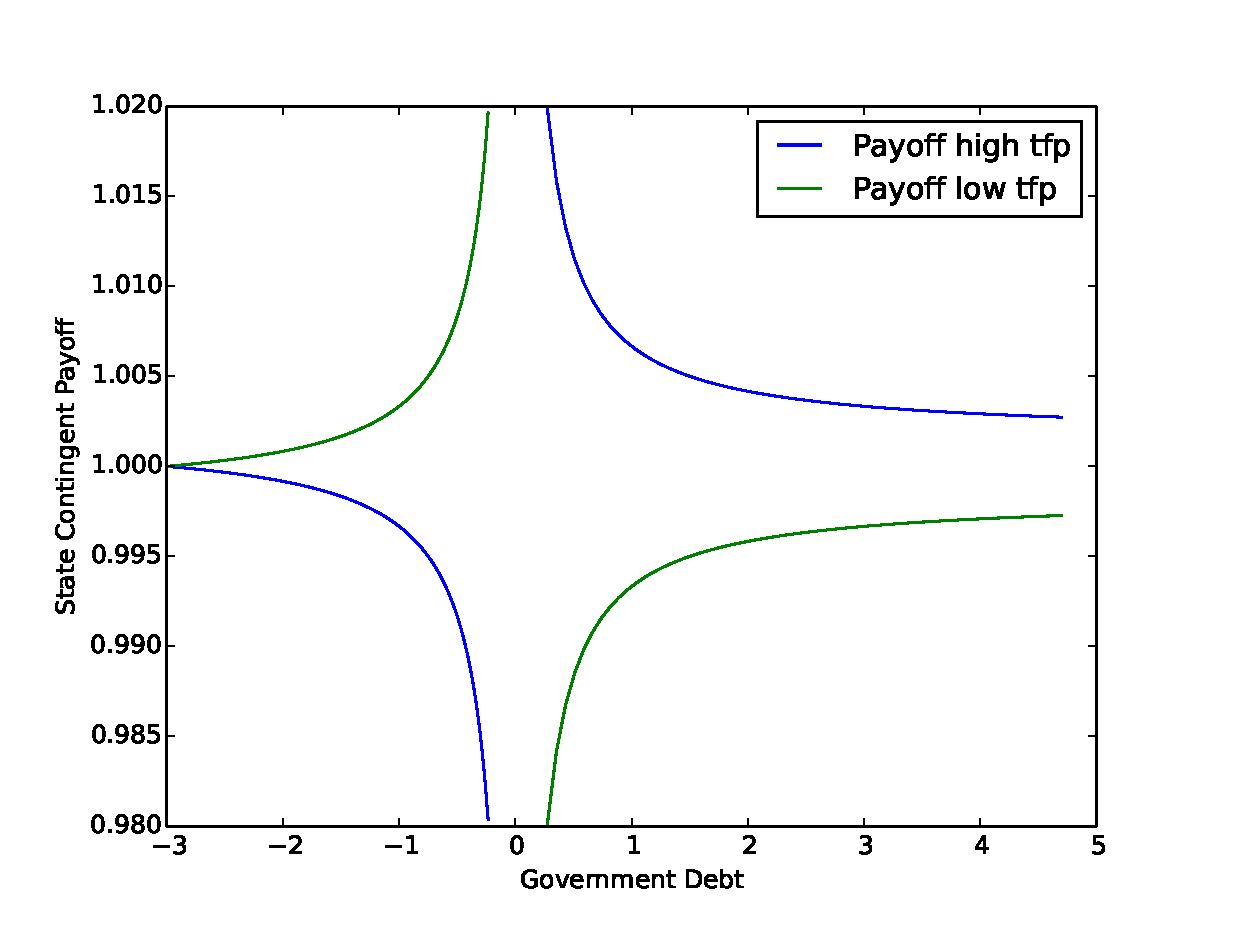
\includegraphics[scale=.4]{Images/p_graph_tfp.eps}
		\caption{Optimal asset payoff structure as a function of initial government debt when TFP follows a 2 shock i.i.d process}
	\end{center}	
	\end{figure}


\begin{figure}
		\begin{center}
		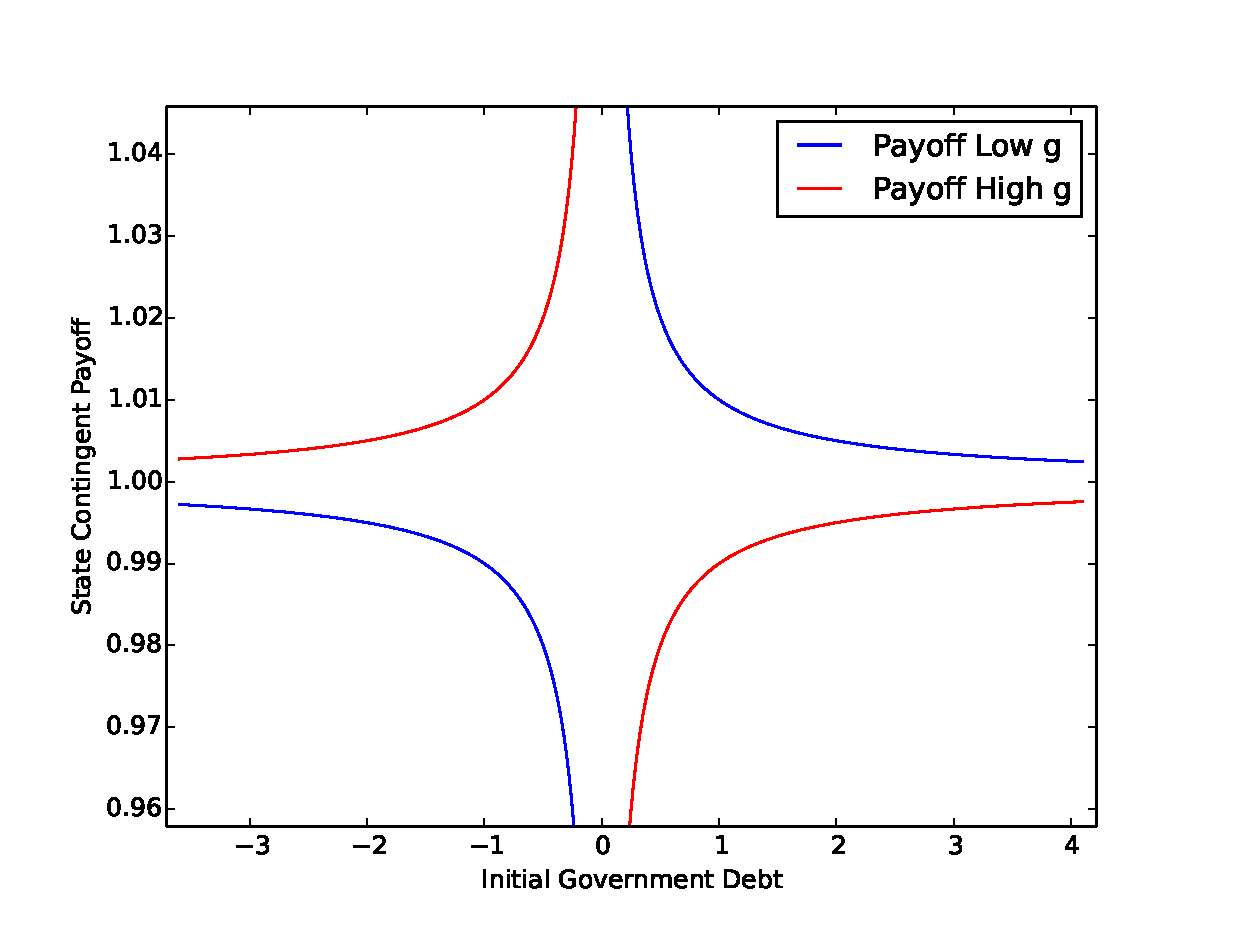
\includegraphics[scale=.4]{Images/p_graph.eps}
		\caption{Optimal asset payoff structure as a function of initial government debt when government expenditures follow 2 shock i.i.d process}
	\end{center}	
	\end{figure}


\begin{figure}
		\begin{center}
		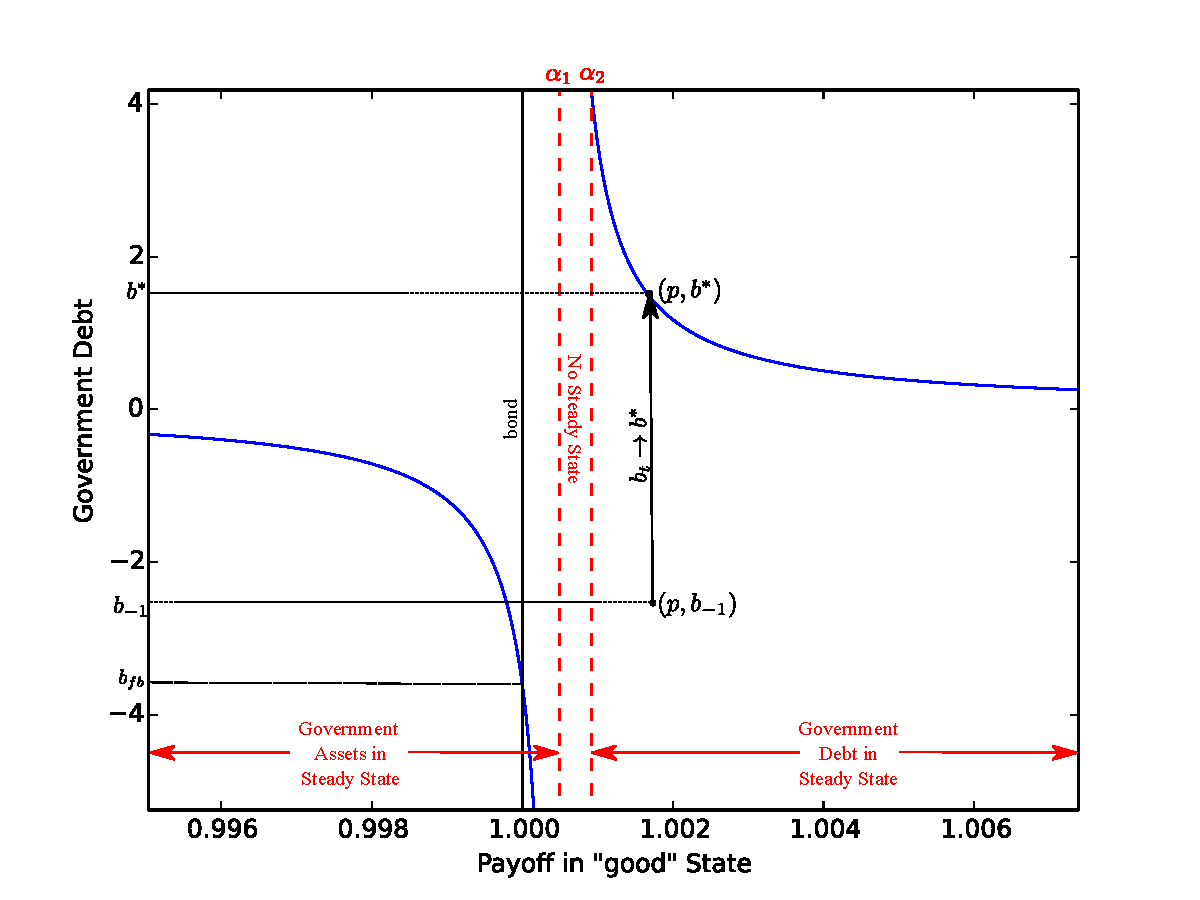
\includegraphics[width=4.2in]{Images/graph_nostable.pdf}
\caption{Existence regions in $\bm{p}$ space}
	\end{center}	
	\end{figure}



	\begin{figure}
		\begin{center}
		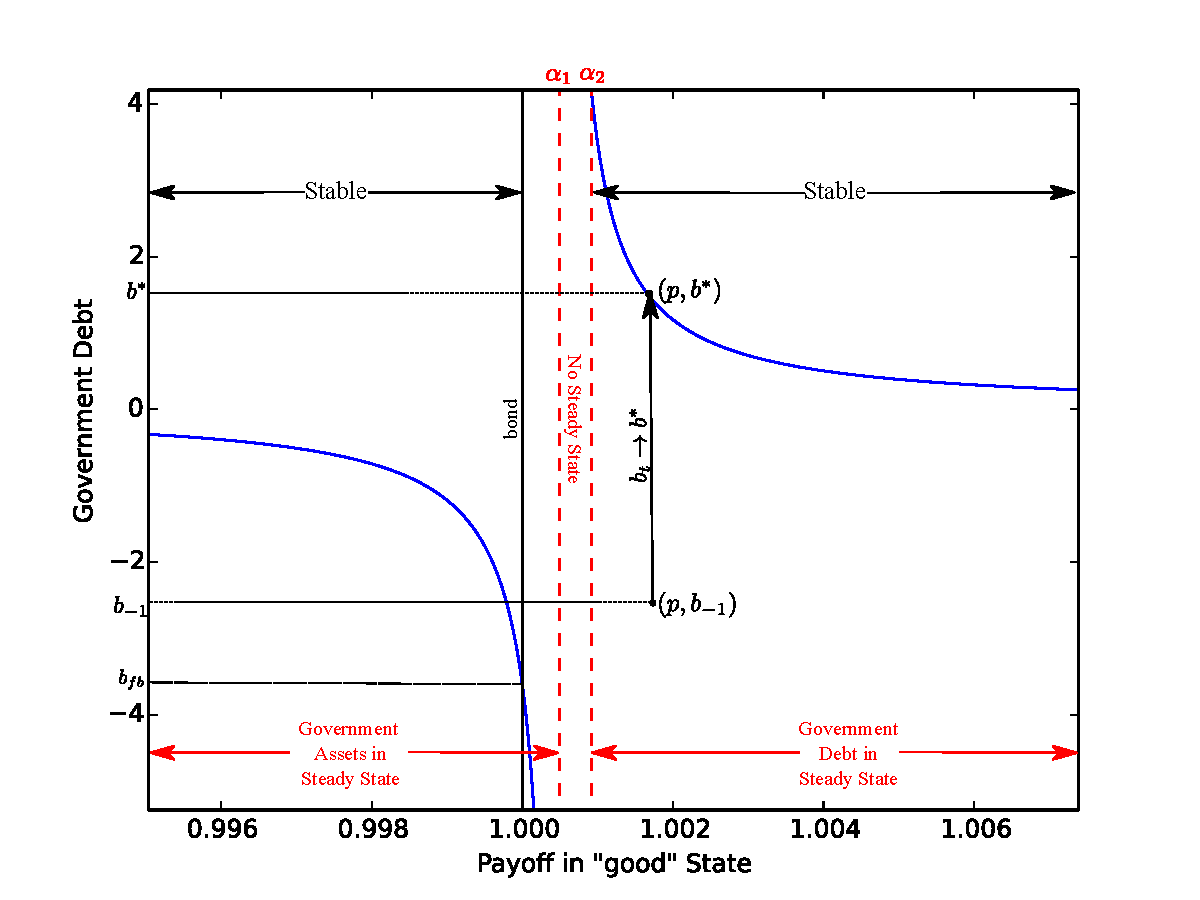
\includegraphics[width = 4.2in]{Images/graph_stable.pdf}
\caption{Stability regions}
	\end{center}	
	\end{figure}	

\begin{figure}
	\begin{center}
	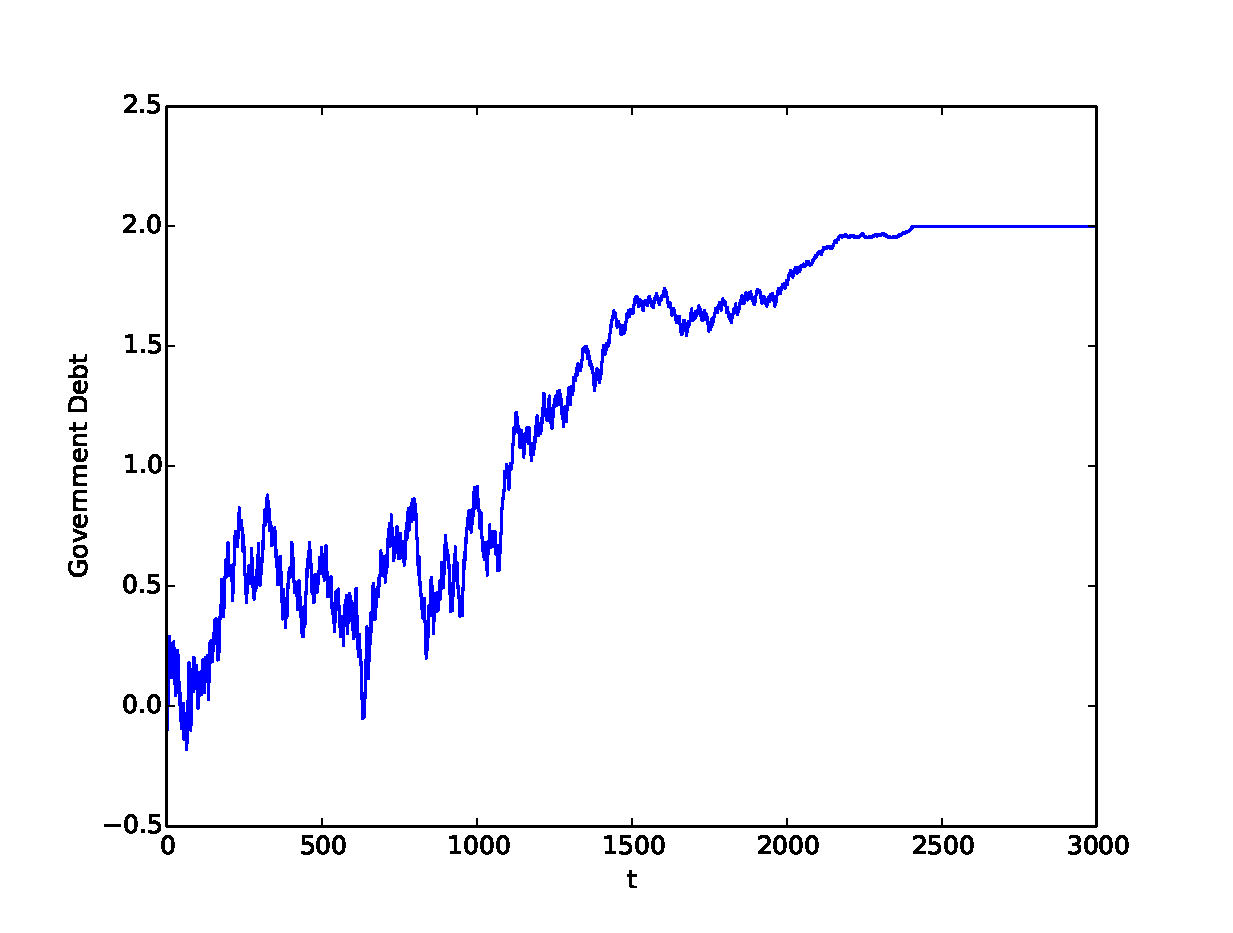
\includegraphics[width=4in]{Images/port1.eps}
    \caption{A sample path with  $\bm{p} > 1$}
	\end{center}
\end{figure}

\begin{figure}
	\begin{center}
	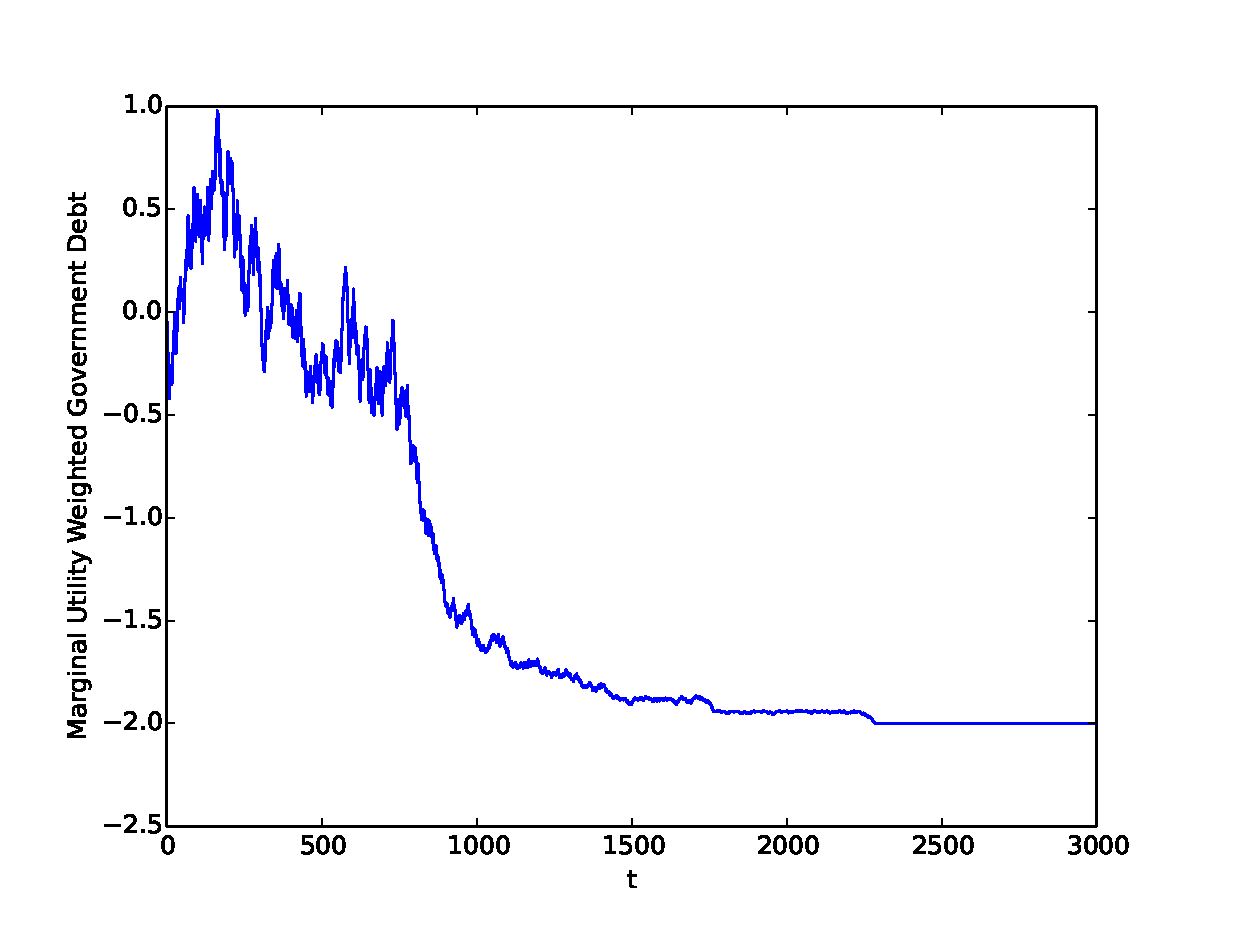
\includegraphics[width=4in]{Images/port2.eps}
\caption{A sample path with   $\bm{p} <1$}
	\end{center}	
\end{figure}



\begin{figure}
	\begin{center}
	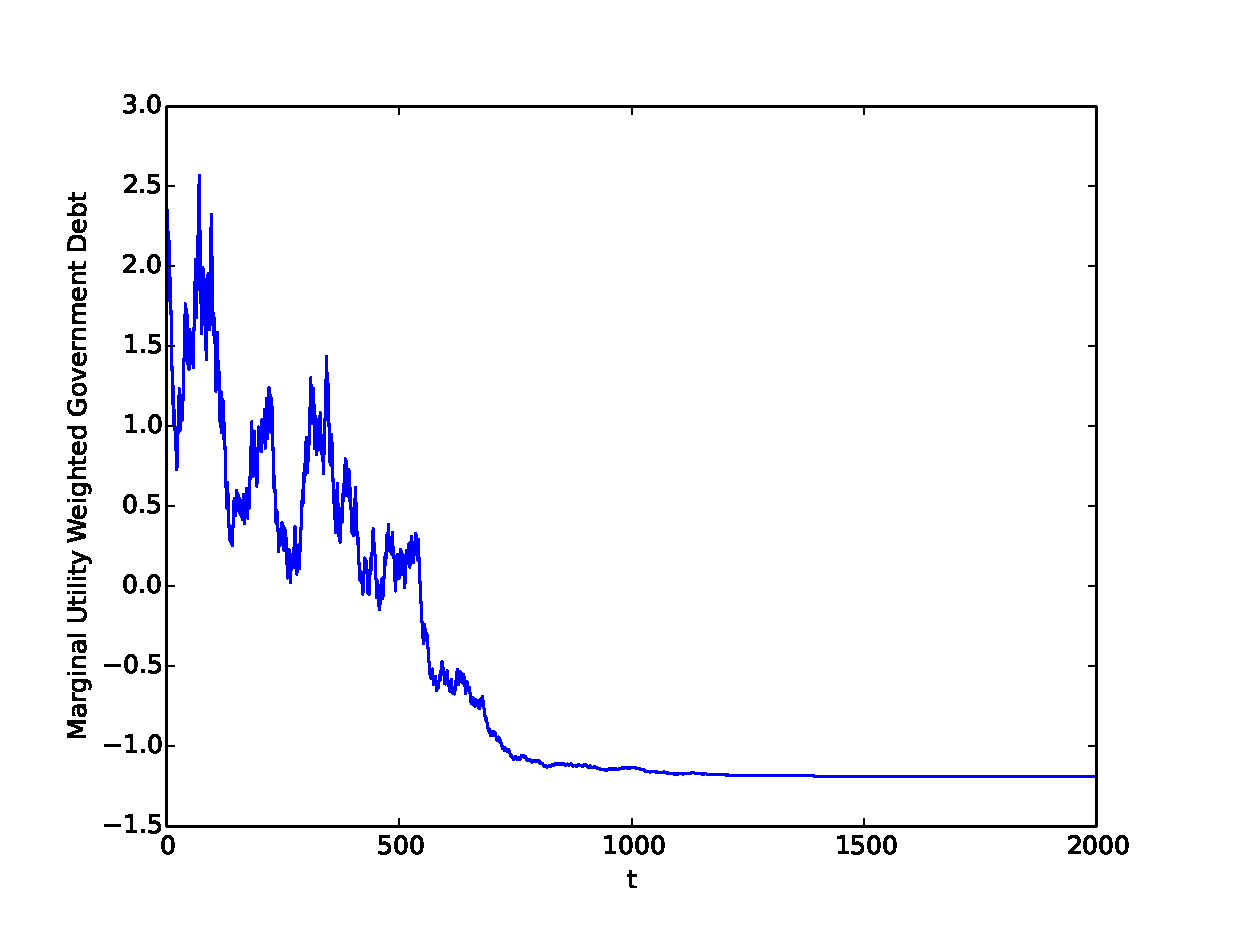
\includegraphics[width=4in]{Images/2stateiid.eps}
\caption{A sample path for 2 state i.i.d. process with risk aversion}
	\end{center}
\end{figure}


	\begin{figure}
	\begin{center}
	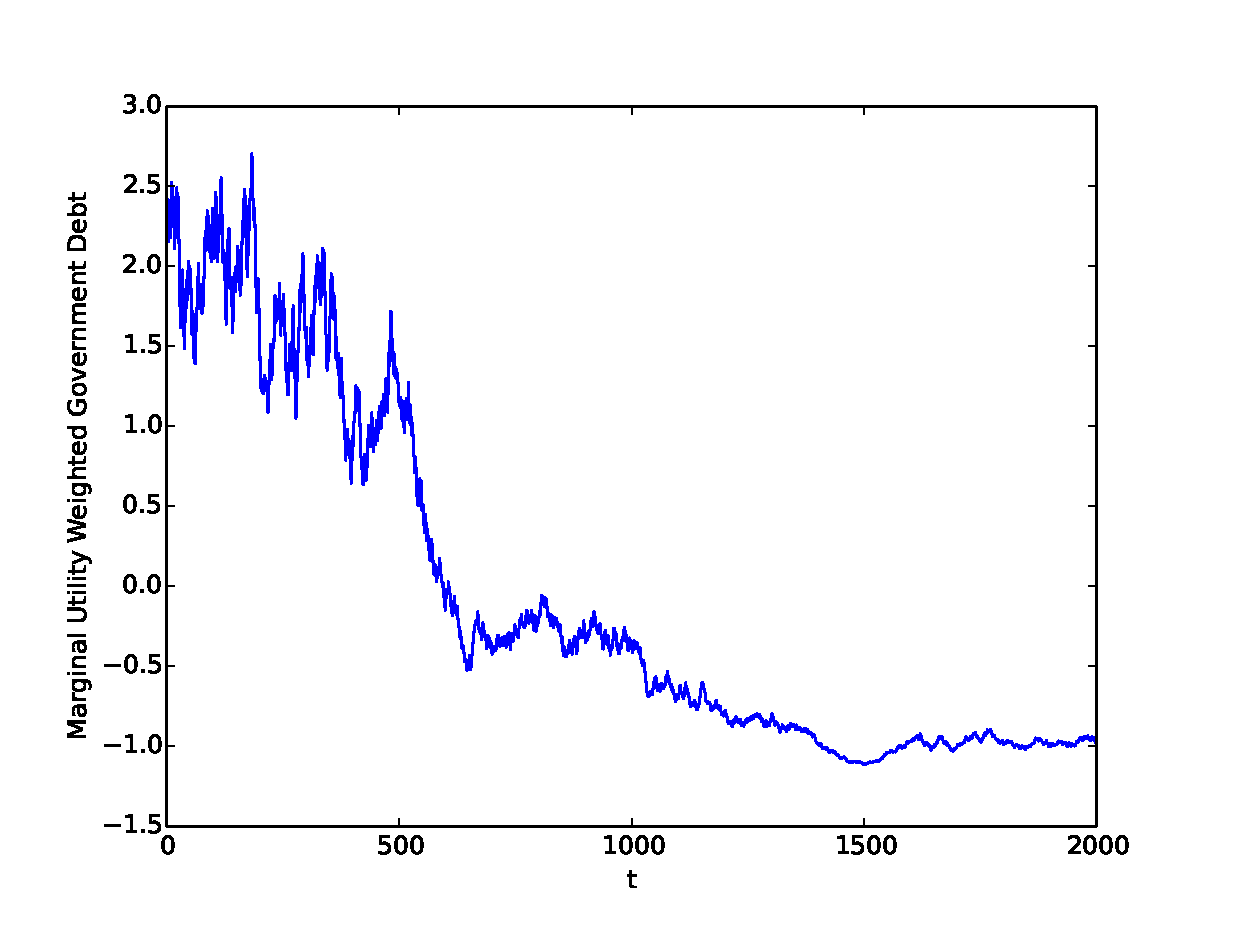
\includegraphics[width=4in]{Images/5stateiid.eps}
\caption{A sample path  for economy with $S>2$ states}
	\end{center}
\end{figure}



\begin{figure}
	\begin{center}
	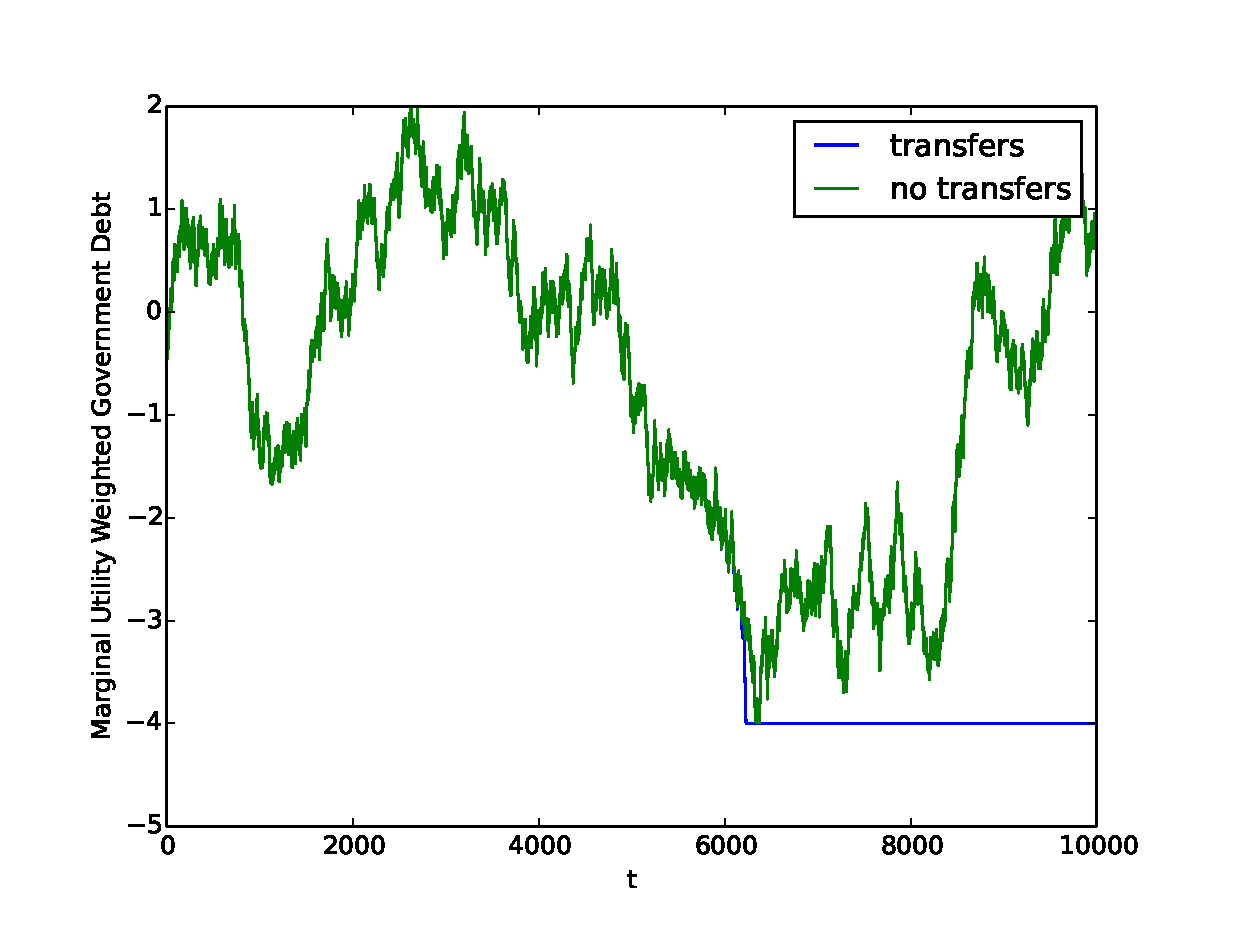
\includegraphics[width=4in]{Images/transfer_example2.eps}
\caption{Quasilinear preferences and risk-free bond  with and without nonnegative transfers}
	\end{center}
\end{figure}



 \end{enumerate}

\bibliography{BEGS}

\end{document}
